\chapter{Perancangan}
\label{chap:perancangan}

Pada bab ini akan dibahas mengenai perancangan perangkat lunak. Perancangan perangkat lunak akan mencakup algoritma, perancangan antarmuka, diagram kelas lengkap, dan perancangan berorientasi objek.

\section{Algoritma}

Pada bagian ini akan berisi mengenai algoritma yang digunakan oleh perangkat lunak dalam menyimpan \textit{password} (\textit{sharing the secret}) and mengembalikan \textit{password} (\textit{reconstructing the secret}). Diasumsikan bahwa sekumpulan pertanyaan keamanan yang logis dengan jawabannya serta \begin{math}n\end{math} (banyak pertanyaan keamanan) dan \begin{math}k\end{math} (banyak minimal jawaban benar yang harus dijawab untuk mengembalikan \textit{password}) sudah ditentukan.

\begin{flushleft}
	\textbf{Algoritma untuk menyimpan \textit{password} \begin{math}p\end{math}}
\end{flushleft}

\begin{enumerate}[label={(\arabic*)}]
	\item Membuat pertanyaan \begin{math}q_1, q_2, ..., q_n\end{math}.
	\item Menjawab setiap pertanyaan \begin{math}q_1, q_2, ..., q_n\end{math} untuk menghasilkan jawaban \begin{math}a_1, a_2, ..., a_n\end{math}.
	\item Menghitung nilai hash \textit{dari} gabungan pertanyaan, jawaban, dan angka acak dinamakan \textit{salt}: \begin{math}h_1 = H(q_1+a_1+r_s), ..., h_n = H(q_n+a_n+r_s)\end{math}.
	\item Membagi \begin{math}p\end{math} menjadi beberapa karakter, kemudian setiap karakter akan diubah menjadi nilai ASCII: \begin{math}c_1, c_2, ..., c_m\end{math}.
	\item Untuk setiap karakter \begin{math}c_1, c_2, ..., c_m\end{math}, dengan menggunakan skema \textit{threshold(k, n)} membagi setiap karakter \begin{math}c_1, c_2, ..., c_m\end{math} menjadi \begin{math}n\end{math} share \begin{math}s_{11}, s_{12}, ..., s_{mn}\end{math}.
	\item Mengenkripsi setiap \textit{share} \begin{math}s\end{math} dengan nilai \textit{hash} sebagai kunci: \begin{math}E_{h_1}(s_{11}) = c_{11}, E_{h_2}(s_{12}) = c_{12}, E_{h_1}(s_{21}) = c_{21}, ..., E_{h_n}(s_{mn}) = c_{mn}\end{math}.
\end{enumerate}

Nilai \textit{salt} \begin{math}r_s\end{math} sebenarnya tidak terlalu dibutuhkan untuk keamanan. Karena walaupun ada kemungkinan bahwa untuk 2 atau lebih kasus  nilai \textit{hash} \begin{math}h_i\end{math} bisa sama tetapi \begin{math}s_{mn}\end{math} pasti akan berbeda sehingga \begin{math}c_{mn}\end{math} pasti akan berbeda juga. Tapi, untuk lebih lagi menjamin keamanan maka nilai \textit{salt} \begin{math}r_s\end{math} tetap akan digunakan.

\begin{flushleft}
	\textbf{Algoritma untuk mengembalikan \textit{password} \begin{math}p\end{math}}
\end{flushleft}

\begin{enumerate}[label={(\arabic*)}]
	\item Menjawab setiap pertanyaan \begin{math}q_1, q_2, ..., q_n\end{math} yang sama untuk menghasilkan jawaban \begin{math}a'_1, a'_2, ..., a'_n\end{math}.
	\item Menghitung nilai hash \textit{dari} gabungan pertanyaan, jawaban, dan \textit{salt}: \begin{math}h'_1 = H(q_1+a'_1+r_s), ..., h'_n = H(q_n+a'_n+r_s)\end{math}.
	\item Mendekripsi setiap ciphertext \begin{math}c_{11}, c_{12}, ..., c{mn}\end{math} dengan nilai hash sebagai kunci: \begin{math}D_{h'_1}(c_{11}) = s'_{11}, D_{h'_2}(c_{12}) = s'_{12}, D_{h'_1}(c_{21}) = s'_{21}, ..., D_{h'_n}(c_{mn}) = s'_{mn}\end{math}.
	\item Dengan menggunakan skema \textit{threshold(k, n)}, untuk setiap share \begin{math}s\end{math}, jika pertanyaan yang dijawab benar banyaknya sesuai atau lebih dari \begin{math}k\end{math}, maka \begin{math}p\end{math} bisa direkontruksi, jika hanya \begin{math}k-1\end{math} atau kurang pertanyaan yang dijawab benar, maka \begin{math}p\end{math} tidak bisa direkonstruksi.
\end{enumerate}

\section{Perancangan Antarmuka}

Perangkat lunak yang dikembangkan akan memiliki 3 tampilan utama, tampilan untuk menyimpan \textit{password}, tampilan untuk mengembalikan \textit{password}, dan tampilan untuk memilih menyimpan \textit{password} atau mengembalikan \textit{password}.

Gambar \ref{fig:tampilan-awal} menunjukkan tampilan awal yang akan dimunculkan pertama kali untuk memilih menyimpan \textit{password} atau mengembalikan \textit{password}.

%diagram
\begin{figure}[h]
	\centerline{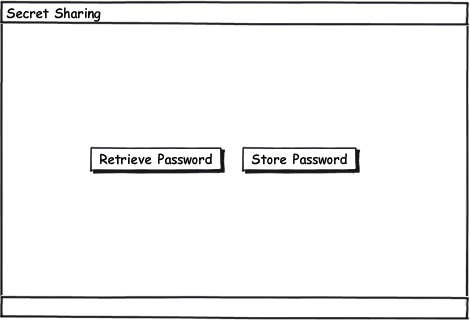
\includegraphics[scale=0.5]{Gambar/tampilan-utama}}
	\caption{Perancangan Tampilan Awal}\label{fig:tampilan-awal}
\end{figure}

Tampilan utama ini cukup sederhana. Dalam tampilan utama pada Gambar \ref{fig:tampilan-awal}, hanya terdapat 2 pilihan, yaitu \textit{store password} untuk menyimpan \textit{password} dan \textit{retrieve password} untuk mengembalikan \textit{password}. Selanjutnya, jika pengguna memilih \textit{store password}, maka akan ditampilkan halaman \textit{store password}.

%diagram
\begin{figure}[h]
	\centerline{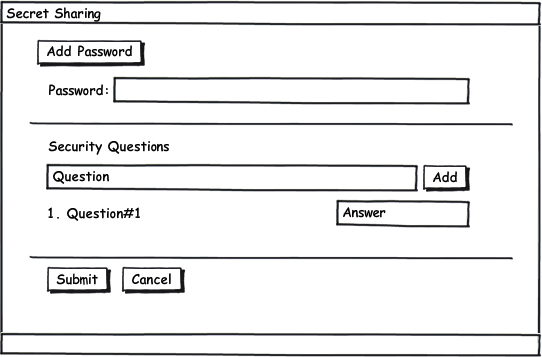
\includegraphics[scale=0.5]{Gambar/store_password}}
	\caption{Perancangan Tampilan Menyimpan \textit{Password}}\label{fig:store_password}
\end{figure}

Pada tampilan menyimpan \textit{password} di Gambar \ref{fig:store_password}, tombol "\textit{Add Password}" berfungsi untuk menambah \textit{text box password}, pada bagian ini pengguna bisa mengisi \textit{password} yang akan disimpan. Bagian "\textit{Security Questions}" berisi pertanyaan keamanan yang dibuat oleh pengguna. Setelah pengguna mengisi pertanyaan personal pada \textit{text box} di bagian "\textit{Security Questions}" dan menekan tombol "\textit{Add}", akan muncul pertanyaan yang sudah dibuat, kemudian pengguna harus mengisi jawaban dari pertanyaan keamanan yang sudah dibuat.

Setelah mengisi seluruh pertanyaan keamanan, pengguna bisa menyimpan \textit{password} dengan menekan tombol "\textit{Submit}". Tombol "\textit{Cancel}" berfungsi untuk kembali ke tampilan awal. Setelah tombol "\textit{Submit}" ditekan, maka \textit{password} sudah disimpan dan akan kembali ditampilkan tampilan awal.

Berikutnya adalah tampilan untuk mengembalikan \textit{password}. Gambar \ref{fig:retrieve_password} menunjukkan tampilan untuk mengembalikan \textit{password}.

%diagram
\begin{figure}[h]
	\centerline{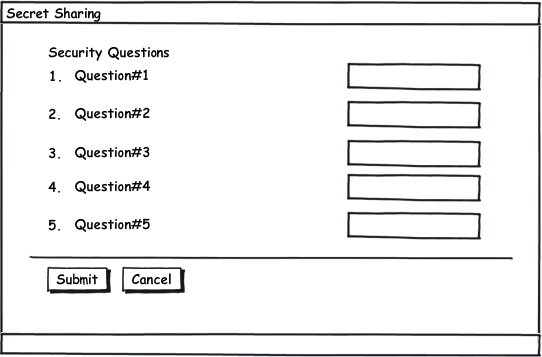
\includegraphics[scale=0.5]{Gambar/retrieve_password}}
	\caption{Perancangan Tampilan Mengembalikan \textit{Password}}\label{fig:retrieve_password}
\end{figure}

Pada bagian untuk mengembalikan \textit{password}, tampilannya cukup sederhana dan pengguna hanya cukup memasukkan setiap jawaban dari pertanyaan keamanan yang sudah dibuat sebelumnya di bagian penyimpanan password. Pada bagian ini, pengguna bebas untuk memilih mengisi setiap pertanyaan atau tidak menjawab pertanyaan keamanan. Setelah seluruh pertanyaan sudah dijawab, pengguna dapat menekan tombol "\textit{Submit}" yang kemudian akan menunjukkan \textit{password} pengguna.

Gambar \ref{fig:password} menunjukkan tampilan sesudah pengguna menekan tombol "\textit{Submit}" pada bagian di Gambar \ref{fig:retrieve_password}.

%diagram
\begin{figure}[h]
	\centerline{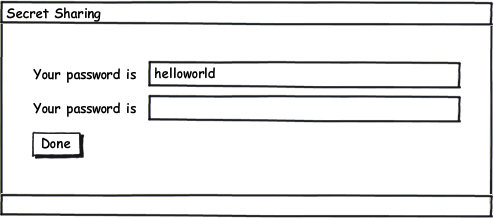
\includegraphics[scale=0.5]{Gambar/password}}
	\caption{Perancangan Tampilan Mengembalikan \textit{Password}}\label{fig:password}
\end{figure}

Jika banyak pertanyaan keamanan yang dijawab benar oleh pengguna sesuai dengan minimal banyak pertanyaan keamanan yang dijawab benar maka pengguna bisa melihat \textit{password} yang sudah disimpan. Tapi, jika banyak pertanyaan keamanan yang dijawab benar oleh pengguna kurang dari minimal banyak pertanyaan keamanan yang harus dijawab benar maka pengguna tidak bisa melihat \textit{password} yang sudah disimpan.

\section{Diagram Kelas Rinci}

Diagram kelas rinci digunakan sebagai gambaran umum untuk setiap kelas yang ada dalam perangkat lunak yang dibangun serta keterkaitan setiap kelas. Diagram kelas rinci dapat dilihat pada Gambar \ref{fig:final_class_diagram}. Ada perbedaan antara diagram kelas pada Gambar \ref{fig:final_class_diagram} dengan kelas diagram pada Bab \ref{chap:analisis}. Pada diagram kelas rinci ditambahkan beberapa atribut dan fungsi sesuai dengan kebutuhan dari masing-masing kelas.

%diagram
\begin{sidewaysfigure}[h]
	\centerline{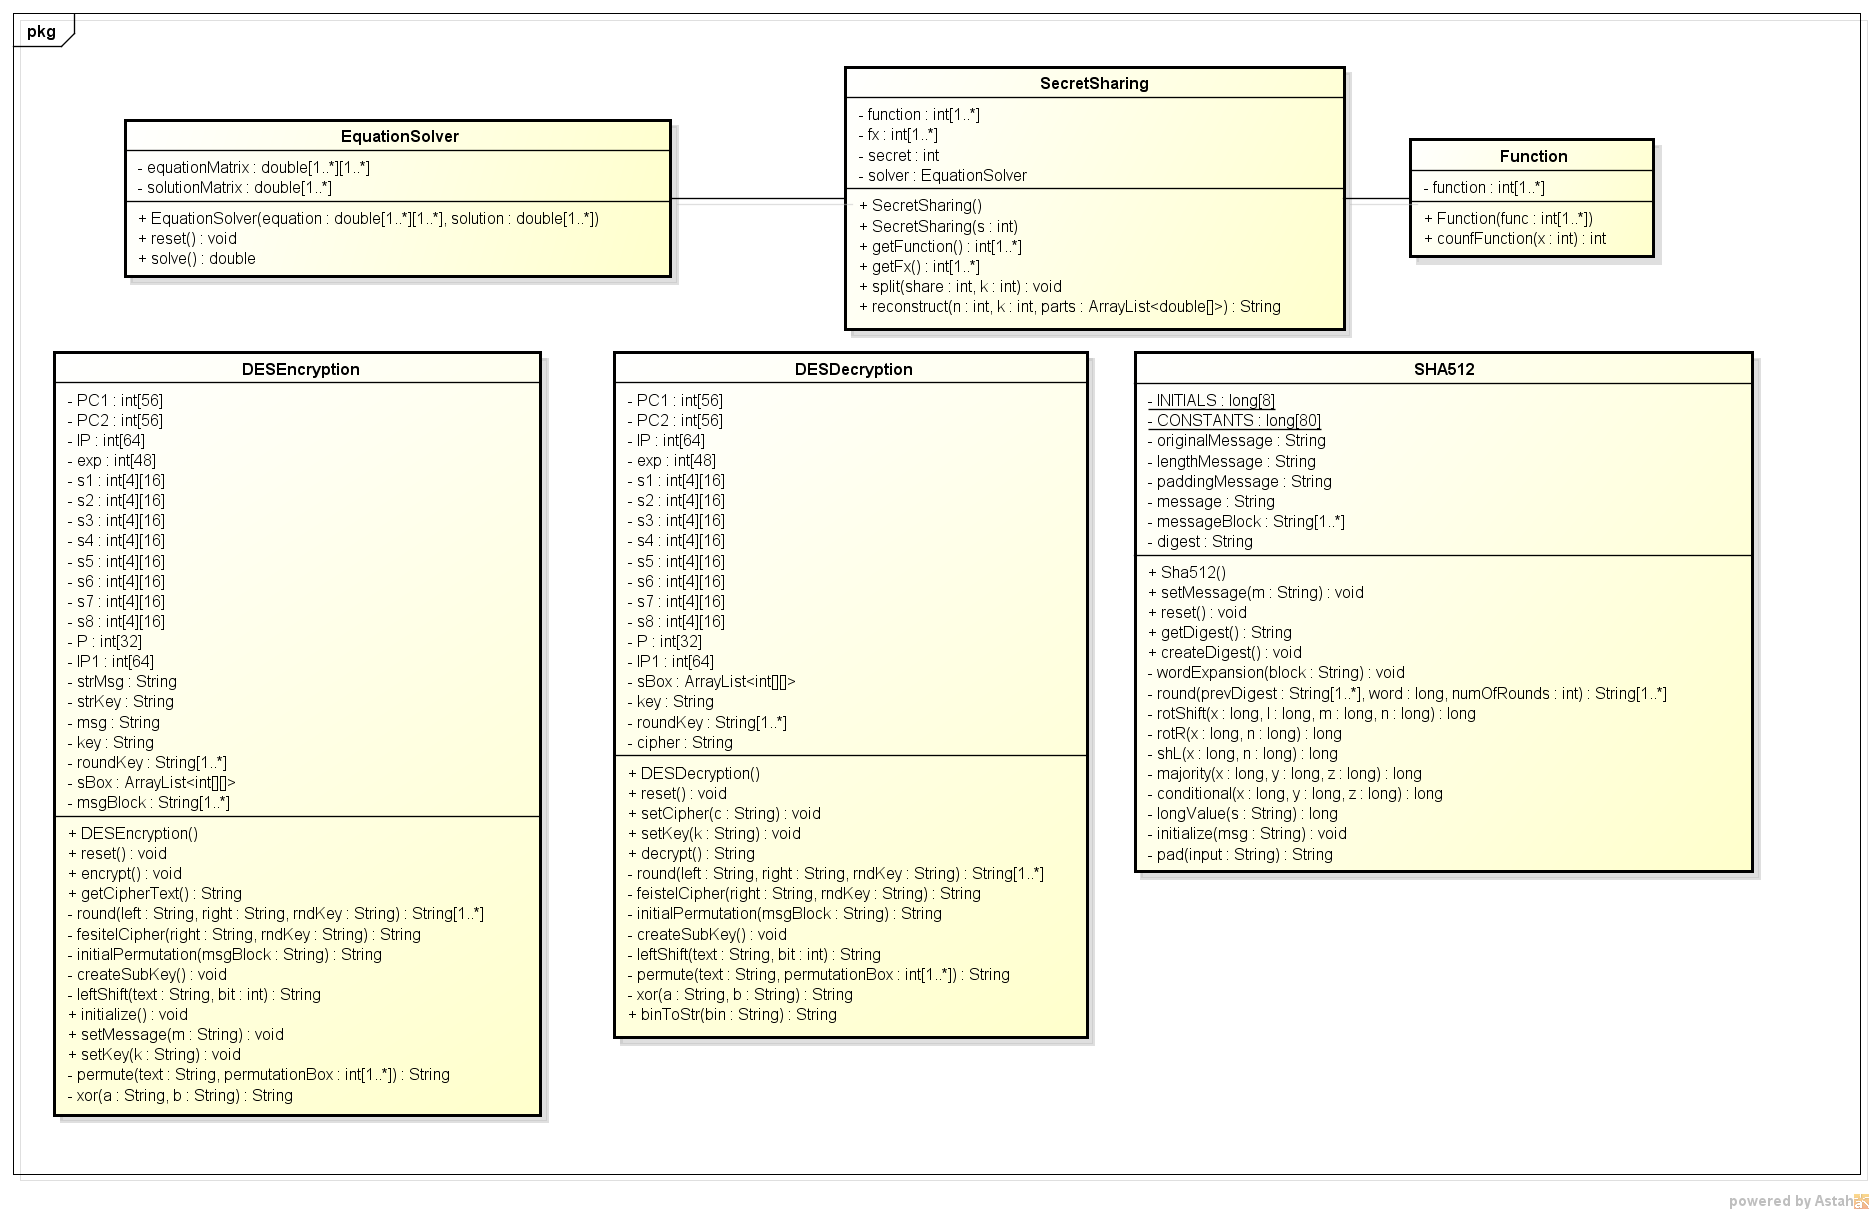
\includegraphics[scale=0.5]{Gambar/final_class_diagram}}
	\caption{Diagram Kelas Rinci}\label{fig:final_class_diagram}
\end{sidewaysfigure}

\section{Deskripsi Kelas dan Fungsi}

Pada bagian ini akan berisi mengenai penjelasan secara rinci masing-masing kelas. Tujuannya adalah menjelaskan peran setiap kelas dalam perangkat lunak yang dibangun.

\subsection{SHA512}

Kelas SHA512 merupakan kelas yang mengimplementasikan \textit{Secure hashing algorithm 512} (SHA-512). Cara kerja algoritma dapat dilihat pada bagian \ref{subsec:SHA512}. Kelas ini memiliki 8 atribut, yaitu \textit{INITIALS, CONSTANTS, originalMessage, lengthMessage, paddingMessage, message, messageBlock,} dan \textit{digest}. Atribut \textit{INITIALS} menyimpan 8 konstanta awal SHA512, dapat dilihat pada gambar \ref{fig:konstanta_sha}. Atribut \textit{CONSTANTS} menyimpan 80 konstanta yang digunakan untuk 80 ronde SHA512.

Atribut \textit{originalMessage} menyimpan \textit{message} dalam bentuk \textit{string}. Atribut \textit{lengthMessage} menyimpan informasi dari panjang atribut \textit{originalMessage} dalam bentuk biner. Atribut paddingMessage menyimpan \textit{padding} dari \textit{originalMessage} dalam bentuk biner. Atribut \textit{message} menyimpan gabungan dari atribut \textit{originalMessage, lengthMessage,} dan \textit{paddingMessage} dalam bentuk biner. Atribut \textit{messageBlock} menyimpan \textit{array} yang berisi \textit{message}, dibagi per 1024-\textit{bit}. Atribut \textit{digest} menyimpan nilai \textit{hash} dari atribut \textit{message}.

Kelas SHA512 memiliki 15 fungsi, yaitu fungsi \textit{setMessage}, fungsi \textit{reset}, fungsi \textit{getDigest}, fungsi \textit{createDigest}, fungsi \textit{wordExpansion}, fungsi \textit{round}, fungsi \textit{rotShift}, fungsi \textit{rotR}, fungsi \textit{shL}, fungsi \textit{majority}, fungsi \textit{conditional}, fungsi \textit{rotate}, fungsi \textit{longValue}, fungsi \textit{initialize}, dan fungsi \textit{pad}.

Fungsi \textit{setMessage} yang berguna untuk mengatur isi dari atribut \textit{message}. Fungsi \textit{reset} berguna untuk mengatur ulang seluruh nilai atribut kecuali untuk atribut \textit{INITIALS} dan \textit{CONSTANTS}. Fungsi \textit{initialize} berguna untuk melakukan inisialisasi awal sebelum menghitung nilai hash, cara kerja fungsi ini bisa dilihat pada bagian Persiapan \textit{Message} dalam \ref{sssec:persiapan_message}.

Fungsi \textit{getDigest} berguna untuk mengembalikan nilai atribut \textit{digest}. Fungsi \textit{rotShift, rotR, shL, majority, conditional,} dan \textit{rotate} merupakan fungsi dasar dari SHA512 yang mengoperasikan \textit{bit-bit}, rumus fungsi ini dapat dilihat pada bagian Ekspansi \textit{Word} dalam \ref{sssec:ekspansi_word} dan Ronde dalam \ref{sssec:rondesha512}. Fungsi \textit{round} merupakan fungsi yang mengimplementasikan satu ronde dalam SHA512, satu ronde dalam SHA512 dapat dilihat pada bagian Ronde dalam \ref{sssec:rondesha512}.

Fungsi \textit{wordsExpansion} merupakan fungsi ekspansi \textit{word} dalam SHA512, cara kerja fungsi ini dapat dilihat pada bagian Ekspansi \textit{Word} dalam \ref{sssec:ekspansi_word}. Fungsi \textit{createDigest} adalah fungsi utama dari kelas SHA512 ini, fungsi ini akan menjalankan 80 ronde dari SHA512 dan menghasilkan nilai \textit{hash} dari atribut \textit{message}. Fungsi \textit{longValue} berguna untuk mengubah nilai \textit{string} menjadi \textit{long}. Fungsi \textit{pad} berguna menambahkan \textit{padding} pada \textit{string} supaya bisa diubah menjadi nilai \textit{long} dengan fungsi \textit{longValue}.

\subsection{\textit{Function}}

Kelas \textit{Function} merupakan kelas yang merepresentasikan sebuah fungsi polinomial \begin{math}f(x)\end{math}. Kelas ini memiliki 1 atribut, yaitu atribut \textit{function} yang menyimpan konstanta setiap koefesien dari fungsi polinomial \begin{math}f(x)\end{math}. Kelas ini memiliki 1 fungsi, yaitu fungsi \textit{countFunction}. Fungsi \textit{countFunction} berguna untuk menghitung nilai dari titik \begin{math}x\end{math} dalam fungsi polinomial \begin{math}f(x)\end{math}.

\subsection{\textit{EquationSolver}}

Kelas \textit{EquationSolver} merupakan kelas yang berguna untuk menyelesaikan persamaan linear. Kelas ini memiliki 2 atribut, yaitu \textit{equationMatrix} dan \textit{solutionMatrix}. Kelas \textit{EquationSolver} memiliki 2 fungsi, yaitu fungsi \textit{reset}, dan fungsi \textit{solve}. Atribut \textit{equationMatrix} menyimpan nilai konstanta setiap koefesien dari matriks persamaan linear. Atribut \textit{solutionMatrix} menyimpan matriks solusi dari persamaan linear. Fungsi \textit{reset} berguna untuk mengembalikan seluruh nilai atribut ke nilai awal. Fungsi \textit{solve} adalah implementasi dari algoritma eliminasi Gauss-Jordan untuk menyelesaikan persamaan linear.

\subsection{\textit{SecretSharing}}

Kelas SecretSharing merupakan kelas yang berperan untuk menjalankan algoritma \textit{secret sharing} shamir. Kelas ini memiliki 4 atribut, yaitu \textit{function, fx, secret,} dan \textit{solver}. Atribut \textit{function} menyimpan konstanta koefesien dari fungsi polinomial \begin{math}f(x)\end{math}. Atribut \textit{fx} menyimpan setiap nilai \begin{math}x\end{math} dari fungsi polinomial \begin{math}f(x)\end{math}. Atribut \textit{secret} menyimpan nilai \textit{secret} dari \textit{share-share} yang akan dibangun. Atribut \textit{solver} menyimpan objek dari kelas \textit{EquationSolver}.

Kelas \textit{SecretSharing} memiliki 4 fungsi, yaitu fungsi \textit{getFunction}, fungsi \textit{getFx}, fungsi \textit{split}, dan fungsi \textit{reconstruct}. Fungsi \textit{getFunction} berguna untuk mengembalikan nilai dari atribut \textit{function}. Fungsi \textit{getFx} berguna untuk mengembalikan nilai atribut \textit{fx}. Fungsi \textit{split} berguna untuk membangun \textit{share-share}. Fungsi \textit{reconstruct} berguna untuk mengembalikan nilai \textit{secret} dari \textit{share-share} yang dimiliki.

\subsection{\textit{DESEncryption}}

Kelas \textit{DESEncryption} merupakan kelas yang mengimplementasikan proses enkripsi algoritma \textit{data encryption standard} (DES). Kelas \textit{DESEncryption} memiliki 22 atribut, yaitu \textit{PC1, PC2, IP, exp, s1, s2, s3, s4, s5, s6, s7, s8, P, IP1, strMsg, strKey, msg, key, roundKey, cipher, sBox,} dan \textit{msgBlock}. Atribut \textit{PC1} dan \textit{PC2} menyimpan matriks permutasi untuk pembangunan kunci ronde. Atribut \textit{IP} menyimpan matriks inisialisasi awal. Atribut \textit{exp} menyimpan matriks ekspansi \textit{P-box}, penjelasan mengenai \textit{P-box} dapat dilihat pada bagian Kompresi \textit{P-box} dalam \ref{sssec:kompresi_Pbox}. Atribut \textit{s1, s2, s3, s4, s5, s6, s7,} dan \textit{s8} menyimpan matriks \textit{S-box}. Atribut \textit{P} menyimpan matriks permutasi untuk setiap ronde dalam DES. Atribut \textit{IP1} menyimpan matriks permutasi akhir.

Atribut \textit{strMsg} menyimpan \textit{plaintext} yang akan dienkripsi. Atribut \textit{strKey} menyimpan kunci rahasia untuk enkripsi. Atribut \textit{msg} menyimpan \textit{plaintext} dalam bentuk biner. Atribut \textit{key} menyimpan kunci rahasia dalam bentuk biner. Atribut \textit{roundKey} menyimpan kunci untuk setiap ronde. Atribut \textit{cipher} menyimpan \textit{ciphertext} hasil enkripsi. Atribut \textit{sBox} menyimpan setiap matriks \textit{S-box}. Atribut \textit{msgBlock} menyimpan \textit{plaintext} dalam bentuk biner yang sudah dibagi menjadi beberapa blok biner berukuran 64-bit.

Kelas \textit{DESEncryption} memiliki 13 fungsi, yaitu fungsi \textit{setMessage}, fungsi \textit{setKey}, fungsi \textit{getCipherText}, fungsi \textit{reset}, fungsi \textit{permute}, fungsi \textit{xor}, fungsi \textit{leftShift}, fungsi \textit{initialize}, fungsi \textit{initialPermutation}, fungsi \textit{createSubKey}, fungsi \textit{feistelCipher}, fungsi \textit{round}, dan fungsi \textit{encrypt}. Fungsi \textit{setMessage} untuk mengatur nilai atribut \textit{strMsg}. Fungsi \textit{setKey} untuk mengatur nilai atribut \textit{strKey}. Fungsi \textit{getCipherText} untuk mengembalikan nilai dari atribut \textit{cipher}. Fungsi \textit{reset} untuk mengatur ulang nilai dari atribut \textit{strMsg, strKey, msg, key, roundKey, cipher,} dan \textit{msgBlock}. Fungsi \textit{permute} merupakan fungsi dasar dalam DES, penjelasan mengenai fungsi ini dapat dilihat pada Tabel \ref{table:permutasi_langsung}.

Fungsi \textit{xor} berguna untuk melakukan operasi \textit{bit xor}. Fungsi \textit{leftShift} berguna untuk menggeser \textit{bit} ke arah kiri sebanyak \begin{math}n\end{math}-\textit{bit}. Fungsi \textit{initialize} berguna untuk memroses \textit{plaintext} dan membangun kunci ronde sebelum dilakukan proses enkripsi. Fungsi \textit{initialPermutation} berguna untuk melakukan permutasi awal. Fungsi \textit{createSubKey} berguna untuk membangun kunci untuk setiap ronde. Fungsi \textit{feistelCipher} merupakan implementasi dari sandi feistel. Fungsi \textit{round} adalah menjalankan satu ronde dari DES. Fungsi \textit{encrypt} merupakan fungsi utama untuk enkripsi menggunakan DES.

\subsection{\textit{DESDecryption}}

Kelas \textit{DESDecryption} merupakan kelas yang mengimplementasikan proses dekripsi algoritma \textit{data encryption standard} (DES). Kelas \textit{DESEncryption} memiliki 18 atribut, yaitu \textit{PC1, PC2, IP, exp, s1, s2, s3, s4, s5, s6, s7, s8, P, IP1, key, roundKey, cipher, sBox,} dan \textit{msgBlock}. Atribut \textit{PC1} dan \textit{PC2} menyimpan matriks permutasi untuk pembangunan kunci ronde. Atribut \textit{IP} menyimpan matriks inisialisasi awal. Atribut \textit{exp} menyimpan matriks ekspansi \textit{P-box}, penjelasan mengenai \textit{P-box} dapat dilihat pada bagian Kompresi \textit{P-box} dalam \ref{sssec:kompresi_Pbox}. Atribut \textit{s1, s2, s3, s4, s5, s6, s7,} dan \textit{s8} menyimpan matriks \textit{S-box}. Atribut \textit{P} menyimpan matriks permutasi untuk setiap ronde dalam DES. Atribut \textit{IP1} menyimpan matriks permutasi akhir.

Atribut \textit{key} menyimpan kunci rahasia untuk dekripsi dalam bentuk biner. Atribut \textit{roundKey} menyimpan kunci untuk setiap ronde. Atribut \textit{cipher} menyimpan \textit{ciphertext} yang akan didekripsi. Atribut \textit{sBox} menyimpan setiap matriks \textit{S-box}. Kelas \textit{DESEncryption} memiliki 12 fungsi, yaitu fungsi \textit{setCipher}, fungsi \textit{setKey}, fungsi \textit{reset}, fungsi \textit{permute}, fungsi \textit{xor}, fungsi \textit{leftShift}, fungsi \textit{binToStr}, fungsi \textit{initialPermutation}, fungsi \textit{createSubKey}, fungsi \textit{feistelCipher}, fungsi \textit{round}, dan fungsi \textit{decrypt}.

Fungsi \textit{setCipher} untuk mengatur nilai atribut \textit{cipher}. Fungsi \textit{setKey} untuk mengatur nilai atribut \textit{key}. Fungsi \textit{reset} untuk mengatur ulang nilai dari atribut \textit{cipher, key,} dan \textit{roundKey}. Fungsi \textit{permute} merupakan fungsi dasar dalam DES, penjelasan mengenai fungsi ini dapat dilihat pada Gambar \ref{table:permutasi_langsung}. Fungsi \textit{xor} berguna untuk melakukan operasi \textit{bit xor}. Fungsi \textit{leftShift} berguna untuk menggeser \textit{bit} ke arah kiri sebanyak \begin{math}n\end{math}-\textit{bit}.

Fungsi \textit{initialPermutation} berguna untuk melakukan permutasi awal. Fungsi \textit{createSubKey} berguna untuk membangun kunci untuk setiap ronde. Fungsi \textit{feistelCipher} merupakan implementasi dari sandi feistel. Fungsi \textit{round} adalah menjalankan satu ronde dari DES. Fungsi \textit{decrypt} menjalankan 16 ronde \textit{inverse} dalam DES.

\subsection{\textit{DataReader}}

Kelas \textit{DataReader} merupakan kelas yang berperan untuk menerima masukkan berupa berkas teks. Kelas ini memiliki 2 atribut, yaitu, \textit{filename} dan \textit{content}. Atribut \textit{filename} menyimpan nama file dari berkas teks yang akan dibaca oleh perangkat lunak. Atribut \textit{content} menyimpan isi dari berkas teks yang dibaca oleh perangkat lunak. Kelas \textit{DataReader} memiliki 2 fungsi, yaitu fungsi \textit{get} dan fungsi \textit{read}. Fungsi \textit{get} berguna untuk mengembalikan nilai dari atribut \textit{content}. Fungsi \textit{read} berguna untuk membaca berkas teks lalu menyimpannya ke dalam atribut \textit{content}.

\subsection{\textit{DataWriter}}

Kelas \textit{DataWriter} merupakan kelas yang berperan untuk menulis keluaran ke dalam berkas teks. Kelas \textit{DataWriter} memiliki 2 atribut, yaitu \textit{filename} dan \textit{content}. Atribut \textit{filename} menyimpan nama berkas teks keluaran akan ditulis. Atribut \textit{content} menyimpan hasil keluaran dari perangkat lunak yang akan ditulis ke dalam berkas teks. Kelas \textit{DataWriter} memiliki 1 fungsi, yaitu fungsi \textit{write}. Fungsi \textit{write} berguna untuk menulis keluaran ke dalam berkas teks.